\documentclass[11pt]{preprint}

\setlength{\topmargin}{0mm} \setlength{\oddsidemargin}{0mm}
\setlength{\textwidth}{160mm} \setlength{\textheight}{215mm}

\usepackage{amssymb,amsmath,amscd,amsthm}
\usepackage{tikz}

\def\enumb{\begin{enumerate}}
\def\enume{\end{enumerate}}
\def\itemb{\begin{itemize}}
\def\iteme{\end{itemize}}
\def\integers{\mathbb{Z}}



\newtheorem{proposition}{Proposition}
\newtheorem{theorem}{Theorem}

\title{Discrete Mathematics, 2016 Fall - Worksheet 8}
\author{Instructor: Zsolt Pajor-Gyulai, CIMS}
\date{October 2, 2016}



\begin{document}

\maketitle

In all of the above problems explain your answer in full English sentences.

\enumb

\item Evaluate the following without doing any writing or arithmetic.
\enumb
\item $\binom{9}{0}=1$
\item $\binom{9}{1}=9$
\item $\binom{9}{8}=9$
\item $\binom{9}{6}-\binom{9}{3}=0$
\item $\binom{0}{0}=1$
\item $\binom{0}{2}=0$
\enume

\item Write out all $3$-element subsets of $\{1,2,3,4,5,6\}$ to verify that $\binom{6}{3}=20$.

\vspace{0.1cm}
\begin{align*}
\{1,2,3\}, \{1,2,4\}, \{1,2,5\}, \{1,2,6\}, \{1,3,4\}, \{1,3,5\},\{1,3,6\},\{1,4,5\},\{1,4,6\}, \{1,5,6\}\\
\{2,3,4\},\{2,3,5\},\{2,3,6\},\{2,4,5\},\{2,4,6\},\{2,5,6\},\\
\{3,4,5\},\{3,4,6\},\{3,5,6\}\\
\{4,5,6\}
\end{align*}
\vspace{0.1cm}
\item Twenty people attend a party. If everyone shakes everyone else's hand exactly once, how many handshakes take place?

\vspace{0.1cm}
The number of handshakes is exactly the number two element subsets of the twenty people and therefore this number is 
\[
\binom{20}{2}
\]
However one can also argue the following way: Every person shakes hand with exactly 19 other people. Since there are twenty of them this would give $20\times 19$ handshakes. However, this counts every handshake exactly twice and therefore the total number of handshakes is
\[
\frac{20\cdot 19}{2}=190.
\]
This also proves $\binom{20}{2}=190$.
\item Prove that 
\[
2^n=\sum_{k=0}^{n}\binom{n}{k}.
\]
One easy way is to substitute $x=y=1$ into the binomial theorem. However, please give a combinatorial proof.

\begin{proof}
We ask the question: how many subsets does an $n$ element set have.

On one hand, we have learned that $|2^{\{1,2,\dots,n\}}|=2^n$. On the other hand the answer is also given by
\[
\sum_{k=0}^{n} \#\{k~element~subsets\}=\sum_{k=0}^{n}\binom{n}{k}
\]
\end{proof}

\item 
\enumb
\item Use the binomial theorem to prove
\[
\binom{n}{0}-\binom{n}{1}+\binom{n}{2}-\binom{n}{3}+\dots\pm\binom{n}{n}=0
\]
\begin{proof}
\[
0=(1-1)=\sum_{k=0}^n\binom{n}{k}1^{n-k}(-1)^{k}=\binom{n}{0}-\binom{n}{1}+\binom{n}{2}-\dots+\binom{n}{n}
\]
\end{proof}
\item Move all the negative terms over to the right hand side to give
\[
\binom{n}{0}+\binom{n}{2}+\binom{n}{4}+\dots=\binom{n}{1}+\binom{n}{3}+\binom{n}{5}+\dots
\]
Give a combinatorial interpretation of this identity.

\begin{proof}
The question we ask: How many subsets does $\{1,\dots,n\}$ have with an even number of elements? Clearly, the LHS gives one answer. To see that the RHS also gives an answer, pick one element and call it 'the chosen one'. For each subset with an even number of elements, we can associate a new subset with an odd number of elements the following way. If 'the chosen one' is in the subset we start with then drop it, if it isn't then add it. Note that the resulting new subsets are all different which means that by counting all the odd element-subsets, we can count all the even elements subsets as well. (This type of argument will be called a bijective proof later.)
\end{proof}
\enume

\newpage
\item Consider the following formula. Give two different proofs one using the factorial formula, the other being a combinatorial proof.
\[
\binom{2n+2}{n+1}=\binom{2n}{n+1}+2\binom{2n}{n}+\binom{2n}{n-1}
\]

\begin{proof}
The right hand side is
\[
\frac{(2n)!}{(n+1)!(n-1)!}+2\frac{(2n)!}{n!n!}+\frac{(2n)!}{(n-1)!(n+1)!}=\frac{(2n)!}{(n+1)!}\left[\frac{2}{(n-1)!}+\frac{2(n+1)}{n!}\right]=
\]
\[
=\frac{(2n)!}{(n+1)!(n+1)!}2[n(n+1)+(n+1)^2]=\frac{(2n)!}{(n+1)!(n+1)!}2(n+1)(2n+1)=\\
\]
\[
=\frac{(2n)!}{(n+1)!(n+1)!}(2n+2)(2n+1)\frac{(2n+2)!}{(n+1)!(n+1)!}=\binom{2n+2}{n+1}
\]

For a combinatorial proof, consider a group of $2n+2$ people and let $i$ and $j$ be two chosen ones. How many ways can be choose a smaller group of $n+1$ people. On one hand, the left hand side gives the answer by definition. On the other hand, one of the following four cases must happen:
\enumb
\item Both $i$ and $j$ are chosen in the smaller group. This can happen $\binom{2n}{n-1}$ ways.
\item Neither $i$ nor $j$ are chosen. This can happen in $\binom{2n}{n+1}$ ways.
\item $i$ is chosen but $j$ is not. This can happen in $\binom{2n}{n}$ ways.
\item $j$ is chosen but $i$ is not. Again, this can happen in $\binom{2n}{n}$ ways.
\enume
The sum of these gives exactly the right hand side.
\end{proof}


\item What is the coefficient of $x^3$ in $(2x-3)^6$?

\vspace{0.1cm}
By the binomial theorem
\[
(2x-3)^6=\sum_{k=0}^6\binom{6}{k}2^kx^k(-3)^{6-k}.
\]
Clearly the $x^3$ term is the one you get by plugging in $k=3$. This coefficient is
\[
\binom{6}{3}2^3(-3)^{6-3}=-20\cdot 8\cdot 27 = 4320
\]
\vspace{0.05cm}
\newpage
\item (Counting lattice paths) Consider a grid such as the one shown in the figure. We want to count the number of paths from the lower left corner to the upper right corner in which each step of the path either goes one unit to the right or one unit upwards (e.g. the bold one on the picture).
)
\begin{figure}[h]
\centering
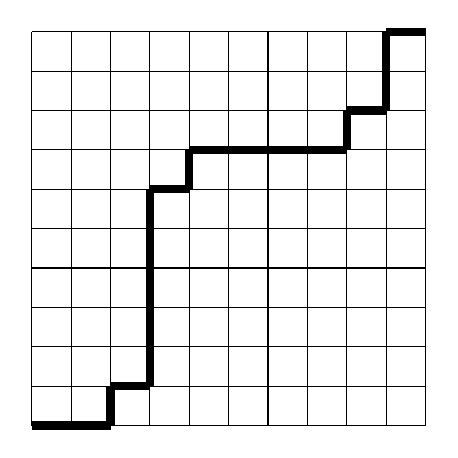
\begin{tikzpicture}[scale=0.5]
\foreach \i in {0,1,2,3,4,5,6,7,8,9,10}
	{
		\draw (\i,0) -- (\i,10);
	}
	
\foreach \i in {0,1,2,3,4,5,6,7,8,9,10}
	{
		\draw (0,\i) -- (10,\i);
	}
	
\draw[line width=3pt] (0,0) -- (2,0);
\draw[line width=3pt] (2,0) -- (2,1);
\draw[line width=3pt] (2,1) -- (3,1);
\draw[line width=3pt] (3,1) -- (3,6);
\draw[line width=3pt] (3,6) -- (4,6);
\draw[line width=3pt] (4,6) -- (4,7);
\draw[line width=3pt] (4,7) -- (8,7);
\draw[line width=3pt] (8,7) -- (8,8);
\draw[line width=3pt] (8,8) -- (9,8);
\draw[line width=3pt] (9,8) -- (9,10);
\draw[line width=3pt] (9,10) -- (10,10);

\end{tikzpicture}
\end{figure}

Every such path consists of exactly 10 rightwards steps and 10 upwards steps. This means that to count these, we have to count how many ways can we choose when to move upwards. Therefore this number is $\binom{20}{10}$.






\item Evaluate the following
\enumb
\item $\binom{3}{1~1~1}=6$
\item $\binom{10}{1~2~5}=0$
\item $\binom{5}{0~5~0}=1$
\item $\binom{10}{7~3~0}=120$
\item $\binom{10}{5~2~3}-\binom{10}{2~3~5}=0$
\enume

\item A coach must choose two teams of 5 from a team of 12 players.  How many different ways can the coach choose the teams?

\vspace{0.1cm}
We have to choose $5$ people to team one, $5$ people to team two and $2$ people are unteamed and so the number we seek is
\[
\binom{12}{5~5~2}=16632
\]

%\item (EXTRA PROBLEM: Computational cost of binomial coefficient) To compute $\binom{n}{k}$ by generating Pascal's triangle, it is not necessary to generate the entire triangle down to row $n$; you need only the part of the triangle in a $90$ degree wedge above $\binom{n}{k}$. Estimate how many additions you would need to perform to calculate $\binom{100}{30}$ by this method.
\enume

\end{document}